\section{Procedimentos}

\par Para que esta pesquisa fosse levada a cabo, tornou-se necessário a implementação de algumas ações, as quais serão detalhadas.

\par O início da pesquisa deu-se através da escolha do tema, seguido pelo levantamento das tecnologias que seriam utilizadas. A princípio, foi definido um escopo contendo algumas tecnologias que foram ministradas no ambiente acadêmico, o que diminui a curva de aprendizado, no entanto, foi preciso agregar alguns conhecimentos novos, onde foi desprendido um tempo a mais para estudo e realização de pequenos testes. As tecnologias que foram empregadas no desenvolvimento deste trabalho são as seguintes: a linguagem de programação JAVA, o banco de dados orientado a grafos Neo4j, juntamente com a API Cypher, Tomcat, Primefaces e JSF, sendo que no decorrer do desenvolvimento prático, viu-se a necessidade de substituir as duas ultimas tecnologias citadas pelas linguagens HTML, CSS, Javascript e Angular JS. As tecnologias que acompanharam o desenvolvimento deste trabalho até a sua conclusão estão descritas no quadro teórico desta pesquisa.

\par Para garantir que as tecnologias selecionadas seriam a melhor escolha no desenvolvimento deste trabalho, foram realizados alguns testes por meio de aplicações simples. Os testes foram focados na avaliação do comportamento do banco de dados orientado a grafos aplicado ao contexto desta pesquisa, cujo objetivo foi desenvolver uma aplicação de busca de mão de obra baseada em uma rede de relacionamentos. Estes testes também foram realizados como fins didáticos, a fim de se familiarizar com as tecnologias utilizadas.

\par Para garantir a qualidade desta pesquisa, o ICONIX foi escolhido como a metodologia de desenvolvimento de \textit{software}, desempenhando um papel fundamental na organização do trabalho. Sua abordagem proveu uma sequencia de procedimentos, que foram seguidos conforme o necessário, levando a construção de uma aplicação estável. Como relatado no quadro teórico, foram seguidas as quatro fases definidas pelo ICONIX.

\par Na primeira fase, definida como análise de requisitos, foi realizado o levantamento das informações pertinentes ao desenvolvimento da aplicação. Este levantamento foi realizado por meio da observação do comportamento das pessoas ao realizar essa busca por mão de obra temporária. A partir dai, foram levantadas as principais características, que seriam indispensáveis para o desenvolvimento deste trabalho e criado o modelo de domínio inicial do projeto como demonstra a Figura 15, com base nas informações levantadas. Nesta fase também foram definidas todas as ações que o usuário poderia realizar no sistema, por meio dos casos de uso, conforme a Figura 16.

\newpage
\begin{figure}[h!]
	\centerline{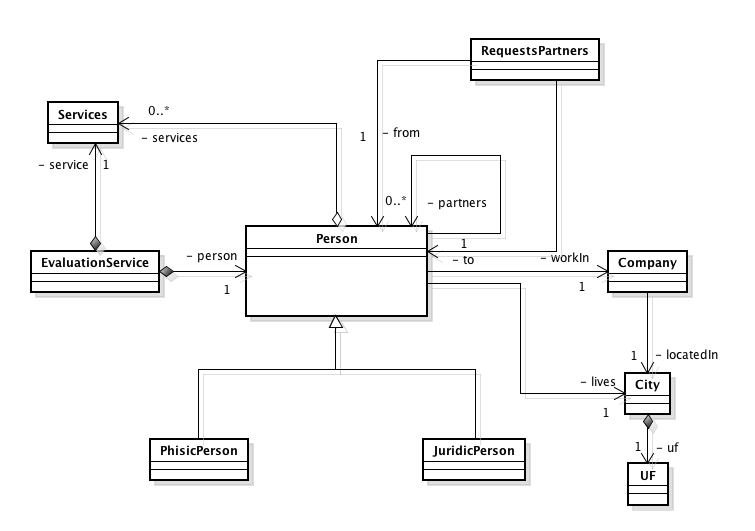
\includegraphics[scale=0.45]{./imagens/modelo-dominio-inicial.png}}
	\caption[Modelo de domínio inicial]
	{Modelo de domínio inicial. \textbf{Fonte:} Elaborado pelos autores.}
	\label{fig:exemplo1}
\end{figure}

\begin{figure}[h!]
	\centerline{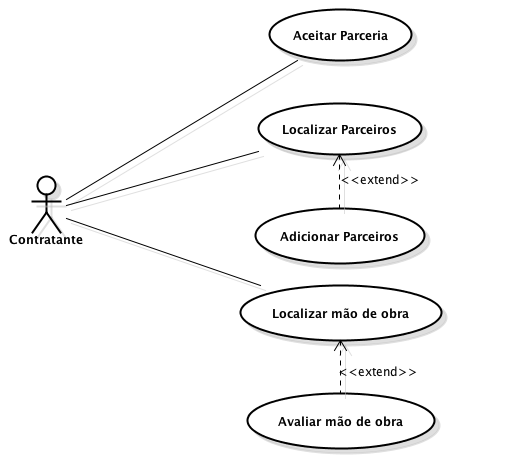
\includegraphics[scale=0.6]{./imagens/caso-de-uso.png}}
	\caption[Diagrama de caso de uso]
	{Diagrama de caso de uso. \textbf{Fonte:} Elaborado pelos autores.}
	\label{fig:exemplo1}
\end{figure}

\par Na segunda fase, análise e projeto preliminar, houve um refinamento dos requisitos levantados na fase anterior, definindo melhor as ações do usuário, por meio dos diagramas de casos de uso. Posterior a esta definição foram gerados os diagramas de robustez, de acordo com os casos de uso definidos, como demonstra a Figura 17. Paralelamente a modelagem desses diagramas, foi atualizado o modelo de domínio, acrescentando os atributos identificados, conforme a Figura 18. Com o modelo de domínio atualizado, foi feita a modelagem do banco de dados da aplicação como apresenta a Figura 19.

\begin{figure}[h!]
	\centerline{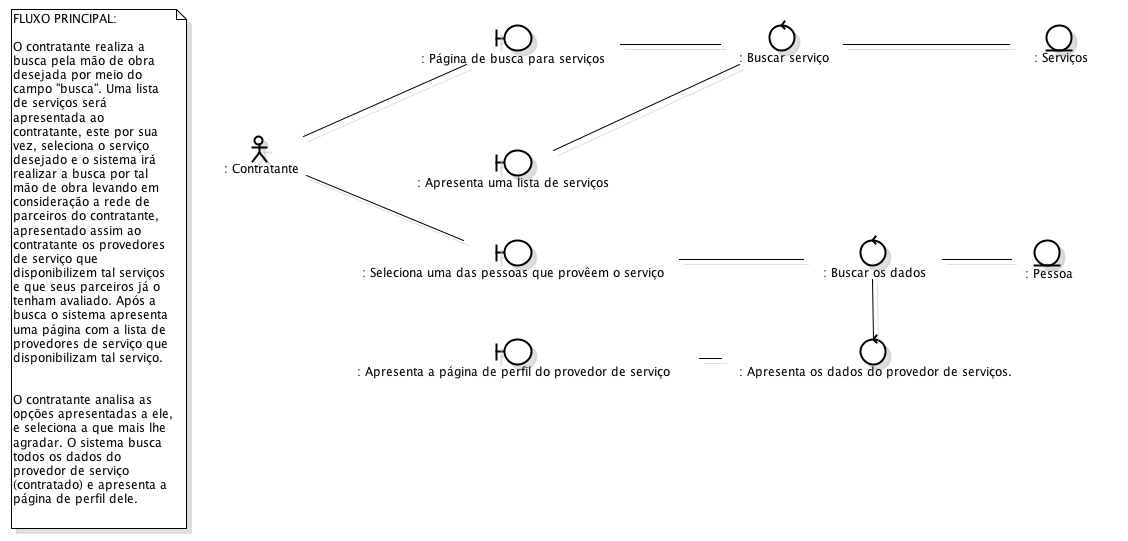
\includegraphics[scale=0.35]{./imagens/robustez.png}}
	\caption[Diagrama de robustez do caso de uso Localizar mão de obra]
	{Diagrama de robustez do caso de uso Localizar mão de obra. \textbf{Fonte:} Elaborado pelos autores.}
	\label{fig:exemplo1}
\end{figure}

\begin{figure}[h!]
	\centerline{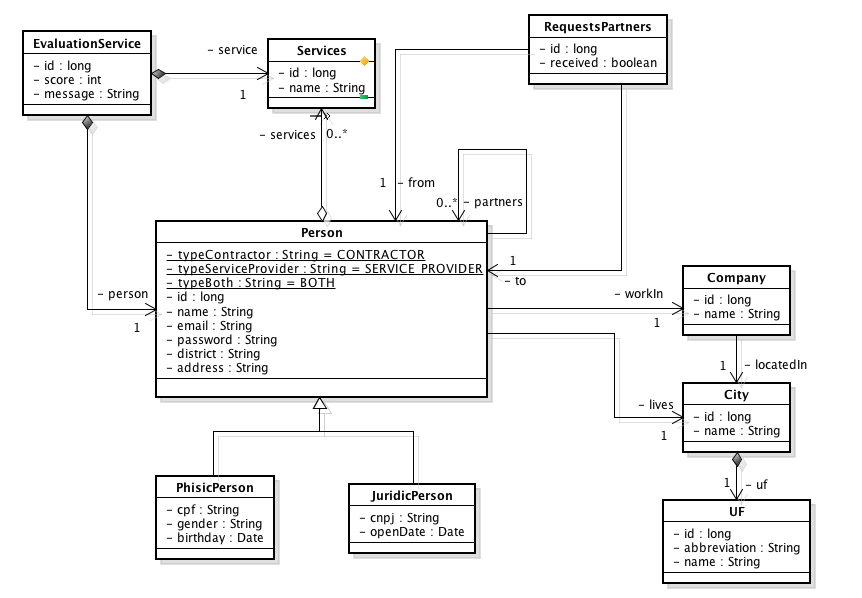
\includegraphics[scale=0.6]{./imagens/modelo-dominio-com-atributos.png}}
	\caption[Modelo de domínio atualizado]
	{Modelo de domínio atualizado. \textbf{Fonte:} Elaborado pelos autores.}
	\label{fig:exemplo1}
\end{figure} 

\begin{figure}[h!]
	\centerline{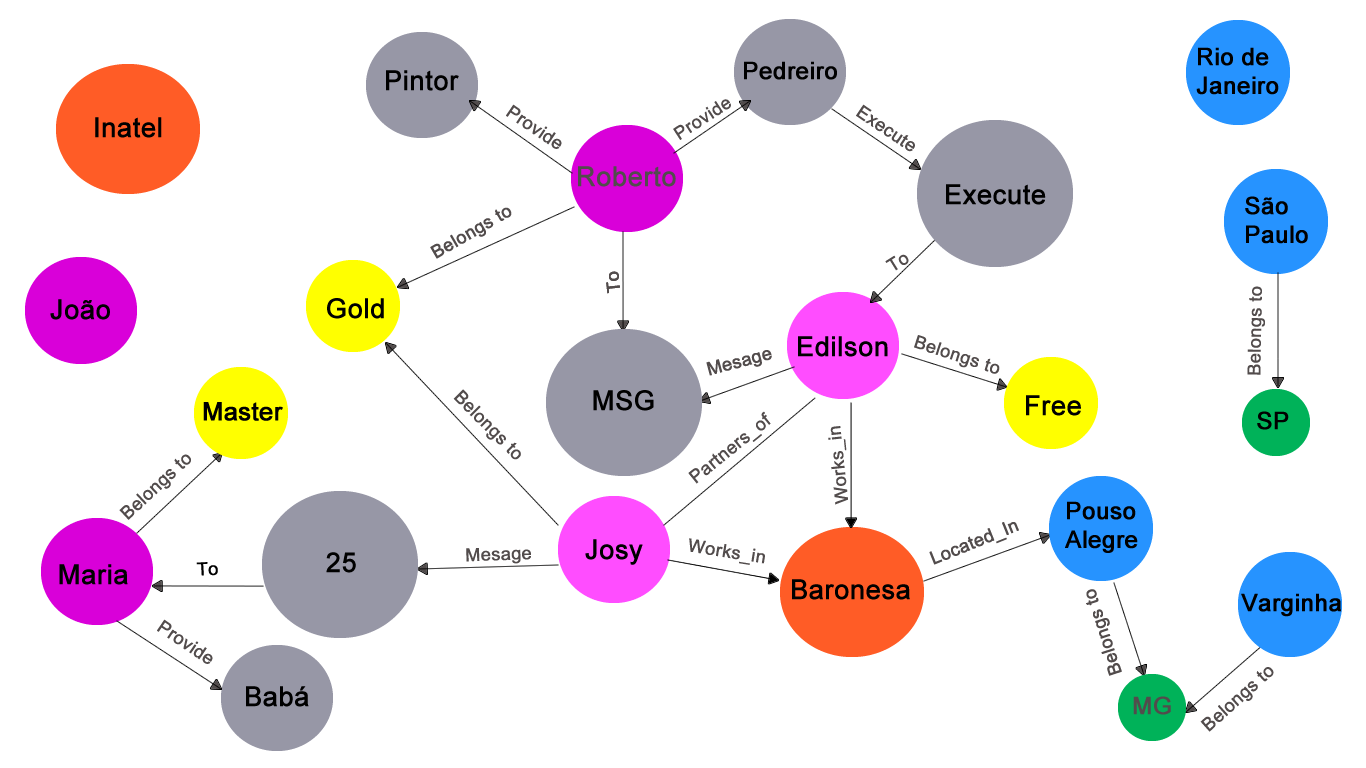
\includegraphics[scale=0.5]{./imagens/structure-all-nodes.png}}
	\caption[Modelo de dados da aplicação]
	{Modelo de dados da aplicação. \textbf{Fonte:} Elaborado pelos autores.}
	\label{fig:exemplo1}
\end{figure} 


\par Na terceira fase, definida como projeto detalhado, foram criados os diagramas de sequencia, tendo como base os casos de uso modelados na fase anterior. Esta fase tem como objetivo detalhar todo o funcionamento do \textit{software}, visando definir a melhor maneira de realizar sua implementação. A Figura 20 apresenta o diagrama de sequência do caso de uso localizar mão de obra.

\newpage
\begin{figure}[h!]
	\centerline{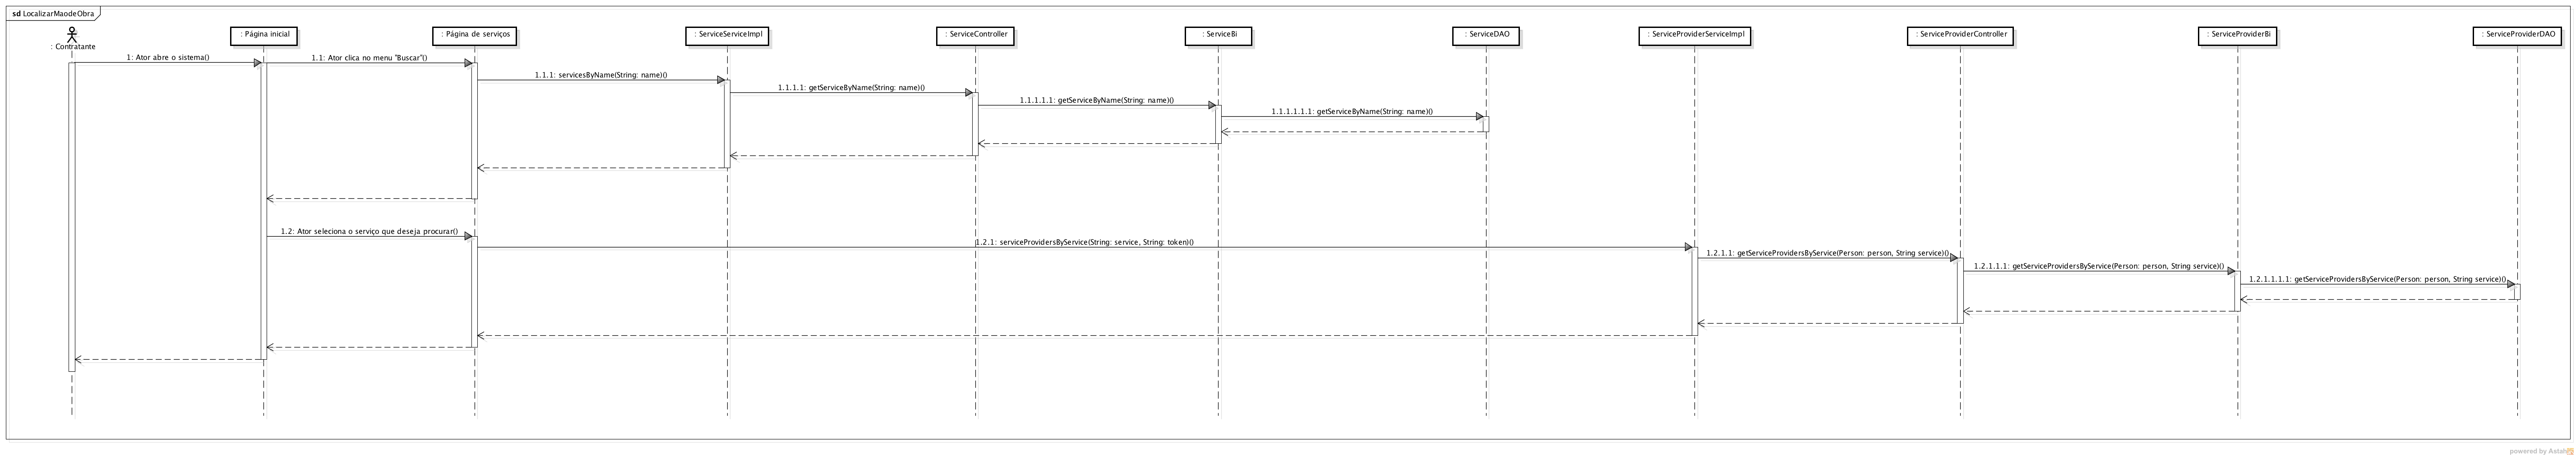
\includegraphics[angle=90,height=0.7\textheight,width=0.7\textwidth]{./imagens/sequence-localizar-mao-de-obra.png}}
	\caption[Diagrama de caso de uso]
	{Diagrama de caso de uso \textbf{Fonte:} Elaborado pelos autores.}
	\label{fig:exemplo1}
\end{figure}

\par Ainda na fase de projeto detalhado, após a modelagem dos diagramas de sequencia, as operações encontradas nestes diagramas foram adicionadas ao modelo de domínio, em conjunto com as novas classes identificadas, gerando assim, o digrama de classes.

imagem do diagrama de classes


\par Na quarta e última fase do ICONIX, denominada implementação, iniciou-se a preparação do ambiente de desenvolvimento, incluindo a instalação de \textit{softwares} adicionais, necessários para o desenvolvimento prático da aplicação.

\par Visto que o trabalho seria desenvolvido em equipe, foi necessário estabelecer uma ferramenta de controle de versão. Esta ferramente permitiu o gerenciamento de diferentes versões de arquivos, gerando um histórico contendo as modificações que foram realizadas no decorrer do processo de desenvolvimento. Este histórico permite o retorno de alguma revisão, caso haja necessidade. A ferramenta escolhida para realizar esse controle foi o GitHub, que já havia sido utilizado em alguns trabalhos do contexto acadêmico, evitando o desprendimento de tempo para estudo de uma nova ferramenta de apoio. O GitHub é uma ferramenta bem difundida e permite que os seus usuários colaborem com os projetos que estão armazenados em seus repositórios\footnotemark[31]. A Figura 21 demonstra a tela de serviços provida pelo GitHub.

\footnotetext[31]{Repositório: local cujo desenvolvedor utiliza para armazenar os documentos relacionados ao \textit{software}.}

\begin{figure}[h!]
	\centerline{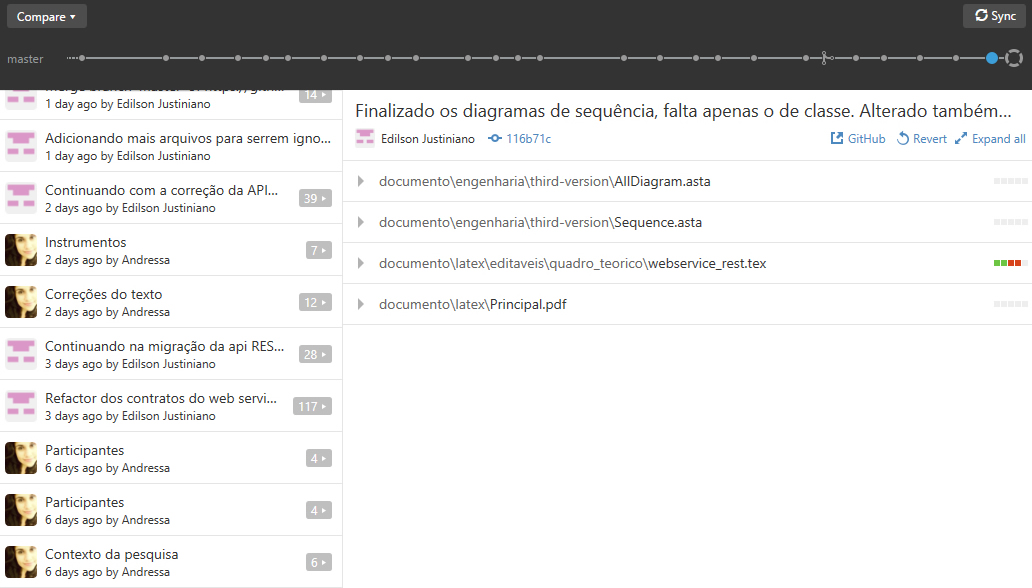
\includegraphics[scale=0.35]{./imagens/github.jpg}}
	\caption[Tela de serviços do GitHub ]
	{Tela de serviços do GitHub \textbf{Fonte:} Elaborado pelos autores.}
	\label{fig:exemplo1}
\end{figure}

\par Os passos de instalação detalhados do GitHub são descritos na sessão apêndices deste trabalho.

\par Como mencionado no quadro teórico, neste trabalho foi utilizada a linguagem Java, sendo assim necessário a utilização de uma IDE de apoio. A IDE escolhida foi o Eclipse, pois se trata de uma ferramenta \textit{open source}, bem difundida no mercado e que permite a escrita de um código mais legível, facilitando tarefas como \textit{debug} e configurações do projeto.

\par O Eclipse possui várias ferramentas, dentre elas, pode-se citar o editor de texto, utilizado não somente para a escrita de códigos em Java, e também a perspectiva de configuração para servidores \textit{web}, utilizada neste trabalho, conforme apresenta a Figura 22. Por meio desta perspectiva, foi configurada a aplicação \textit{container} Tomcat na versão 7.

\newpage
\begin{figure}[h!]
	\centerline{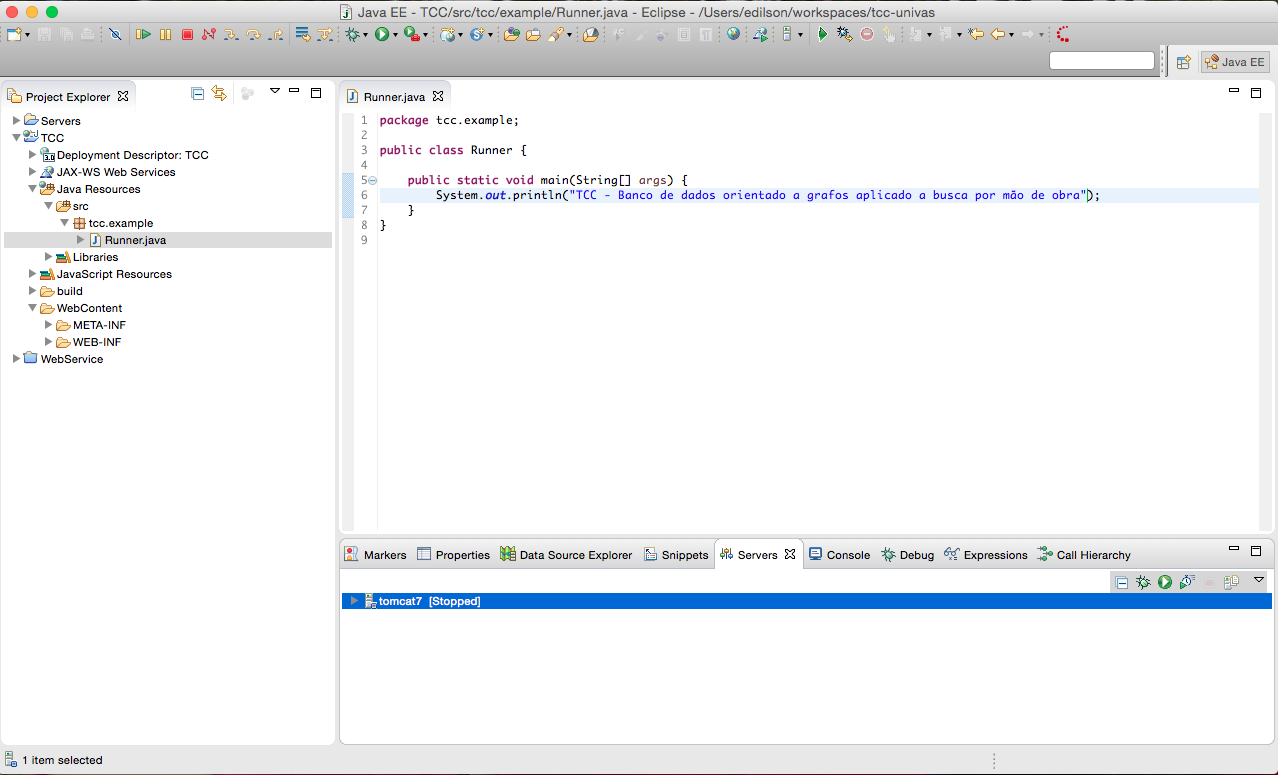
\includegraphics[scale=0.35]{./imagens/eclipse-editor-texto.png}}
	\caption[Ferramentas da IDE Eclipse]
	{Ferramentas da IDE Eclipse \textbf{Fonte:} Elaborado pelos autores.}
	\label{fig:exemplo1}
\end{figure}

\par O Tomcat desempenhou um papel fundamental na execução desta aplicação, pois serviu como hospedeiro para a aplicação Java desenvolvida neste trabalho. 

\par Os passos de instalação e configuração do Eclipse e do Tomcat são descritos na sessão apêndices deste trabalho.

\par Para a escrita do código relacionado ao HTML, CSS e Javascript, foi utilizado o mesmo editor de texto citado anteriormente.

\par O trabalho fez uso de um banco de dados orientado a grafos, o Neo4j. A escolha desse banco se deu pela sua simplicidade de instalação, configuração, facilidade de integração com a API \textit{Cypher} e por disponibilizar uma API REST para acesso aos seus dados, conforme descrito no quadro teórico deste trabalho. O Neo4j faz parte do enquadramento de softwares livres, seguindo o conceito \textit{open source}, o que permite ao desenvolvedor utilizá-lo da forma que melhor lhe convém. 


\par A seguir serão detalhados os passos para a instalação do banco de dados Neo4j.

\par Para realizar o \textit{download} do instalador do banco de dados Neo4j, deve-se acessar a seguinte url, por meio de um  navegador de internet: http://neo4j.com/download e selecionar a opção desejada. Neste trabalho como já descrito foi utilizada a versão \textit{Community}. A Figura 23 apresenta a página de download do Neo4j.

\newpage
\begin{figure}[h!]
	\centerline{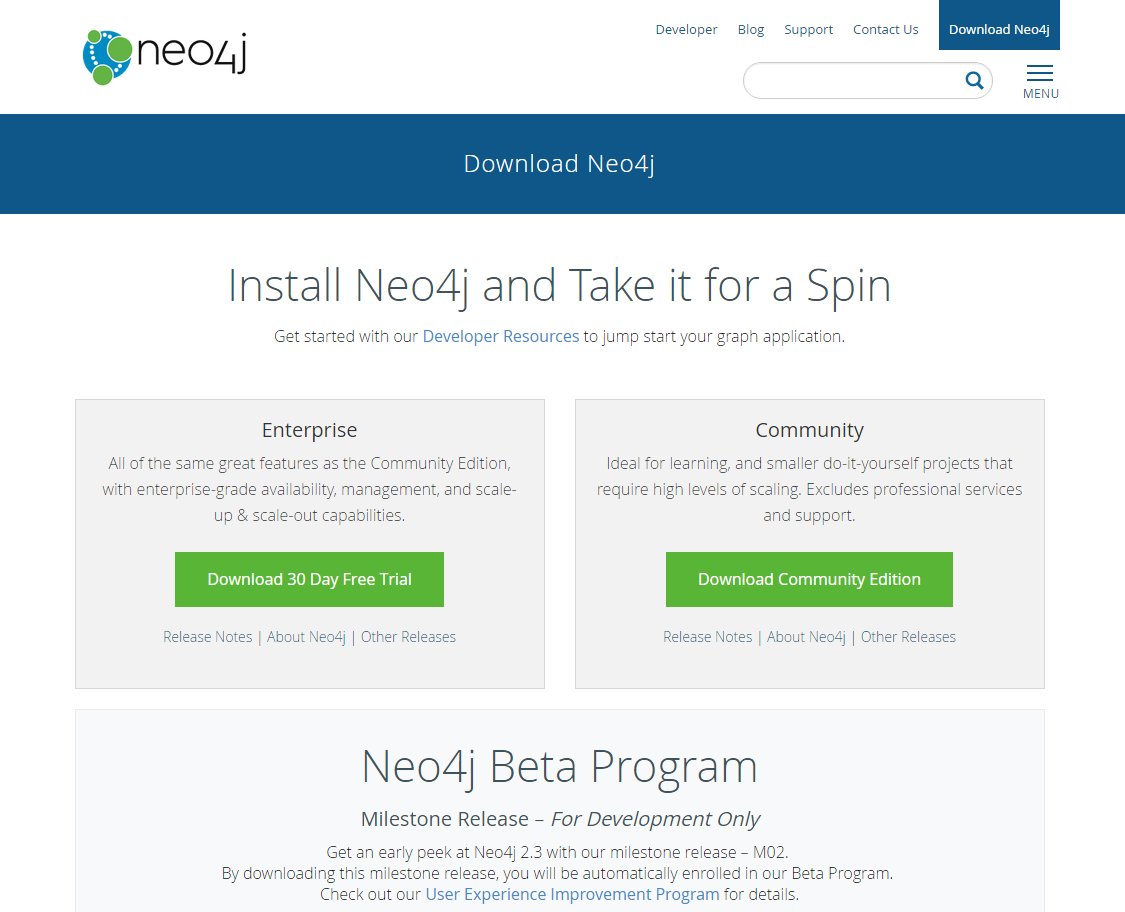
\includegraphics[scale=0.4]{./imagens/download-neo4j.png}}
	\caption[Página de download do Neo4j]
	{Página de download do Neo4j. \textbf{Fonte:} http://neo4j.com/download}
	\label{fig:exemplo1}
\end{figure}

\par Após concluído o \textit{download}, deve-se executar o arquivo. O processo de instalação se inicia e, a primeira tela apresentada ao usuário é a tela contendo uma mensagem de boas vindas, conforme demonstra a Figura 24. Nesta tela, deve-se clicar no botão \textit{Next} para prosseguir com o processo de instalação.

\begin{figure}[h!]
	\centerline{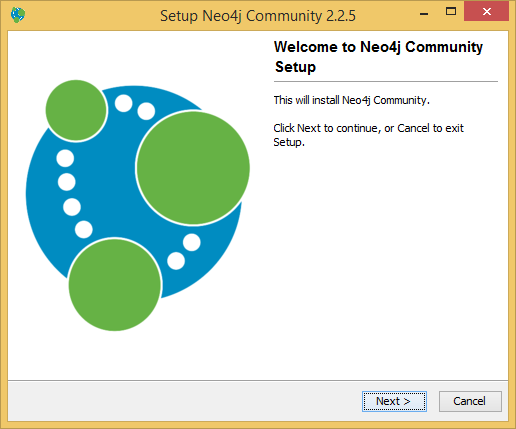
\includegraphics[scale=0.4]{./imagens/neo4j-install-step1.png}}
	\caption[Tela de boas vindas da instalação do Neo4j]
	{Tela de boas vindas da instalação do Neo4j. \textbf{Fonte:} Elaborado pelos autores.}
	\label{fig:exemplo1}
\end{figure}

\par A próxima tela apresentada ao usuário diz respeito ao contrato de uso do \textit{software}, como mostra a Figura 25. Após lê-lo, deve-se aceitar os termos do contrato e clicar no \textit{Next}.

\newpage
\begin{figure}[h!]
	\centerline{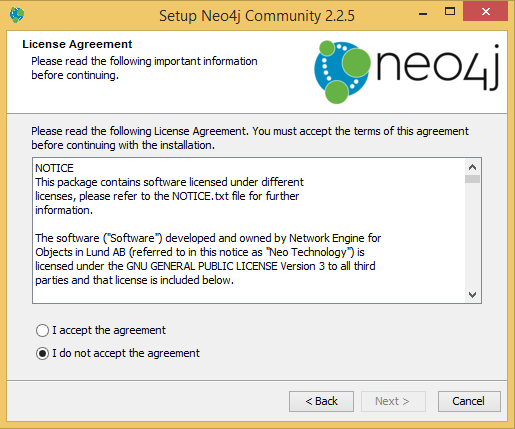
\includegraphics[scale=0.4]{./imagens/neo4j-install-step2.png}}
	\caption[Tela do contrato de uso do Neo4j]
	{Tela do contrato de uso do Neo4j. \textbf{Fonte:} Elaborado pelos autores.}
	\label{fig:exemplo1}
\end{figure}

\par Na próxima tela, conforme a Figura 26 demonstra, é definido o diretório de instalação do Neo4j. Por padrão este diretório é o mesmo das demais aplicações no Windows, podendo ser alterado conforme a necessidade. Após definir o diretório de instalação deve-se clicar no botão \textit{Next}.

\begin{figure}[h!]
	\centerline{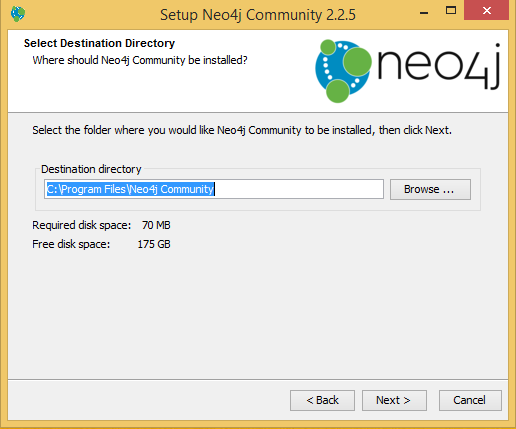
\includegraphics[scale=0.4]{./imagens/neo4j-install-step3.png}}
	\caption[Tela para definição do diretório de instalaão do Neo4j]
	{Tela para definição do diretório de instalaão do Neo4j. \textbf{Fonte:} Elaborado pelos autores.}
	\label{fig:exemplo1}
\end{figure}

\par Após as definições anteriores, uma tela é apresentada questionando ao usuário a respeito da criação de atalhos na área de trabalho, como é demonstrado na Figura 27. Após definir os atalhos do Neo4j, deve-se clicar no botão \textit{Next}.

\begin{figure}[h!]
	\centerline{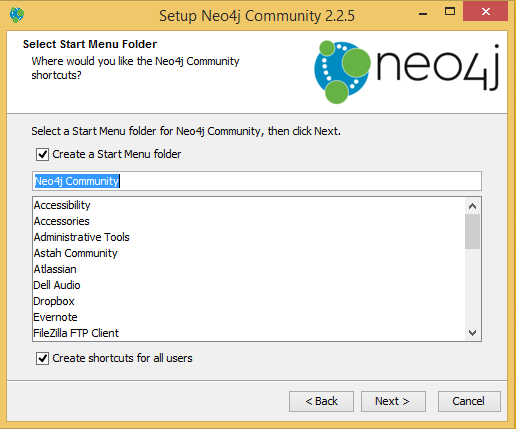
\includegraphics[scale=0.4]{./imagens/neo4j-install-step4.png}}
	\caption[Tela para criação de atalhos do Neo4j]
	{Tela para criação de atalhos do Neo4j. \textbf{Fonte:} Elaborado pelos autores.}
	\label{fig:exemplo1}
\end{figure}

\par Após realizar os procedimentos descritos para a instalação do Neo4j a tela final de instalação será apresentada, informando-o a respeito do resultado da instalação conforme demonstra a Figura 28. Clique no botão \textit{Finish} para finalizar o processo de instalação.
Após todos os passos realizados com sucesso, o Neo4j estará disponível.

\begin{figure}[h!]
	\centerline{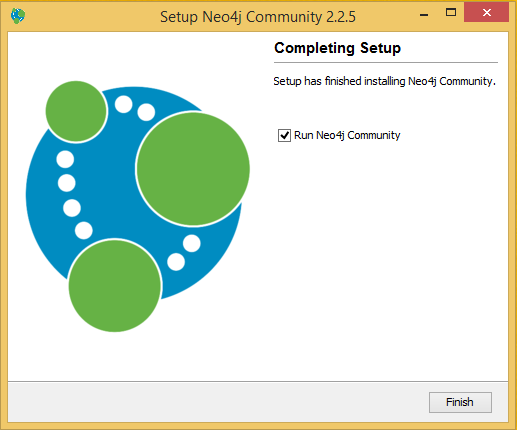
\includegraphics[scale=0.4]{./imagens/neo4j-install-step5.png}}
	\caption[Tela final de instalação do Neo4j]
	{Tela final de instalação do Neo4j. \textbf{Fonte:} Elaborado pelos autores.}
	\label{fig:exemplo1}
	
\end{figure}

\par Depois de concluir a instalação do banco de dados, é necessário realizar a conexão com a aplicação. Para isso foi implementada uma classe em Java, utilizando a API Eclipse, que contém os parâmetros responsáveis por executar a conexão. A Figura 29 mostra o trecho de código responsável por valiar esta conexão.


\begin{figure}[h!]
	\centerline{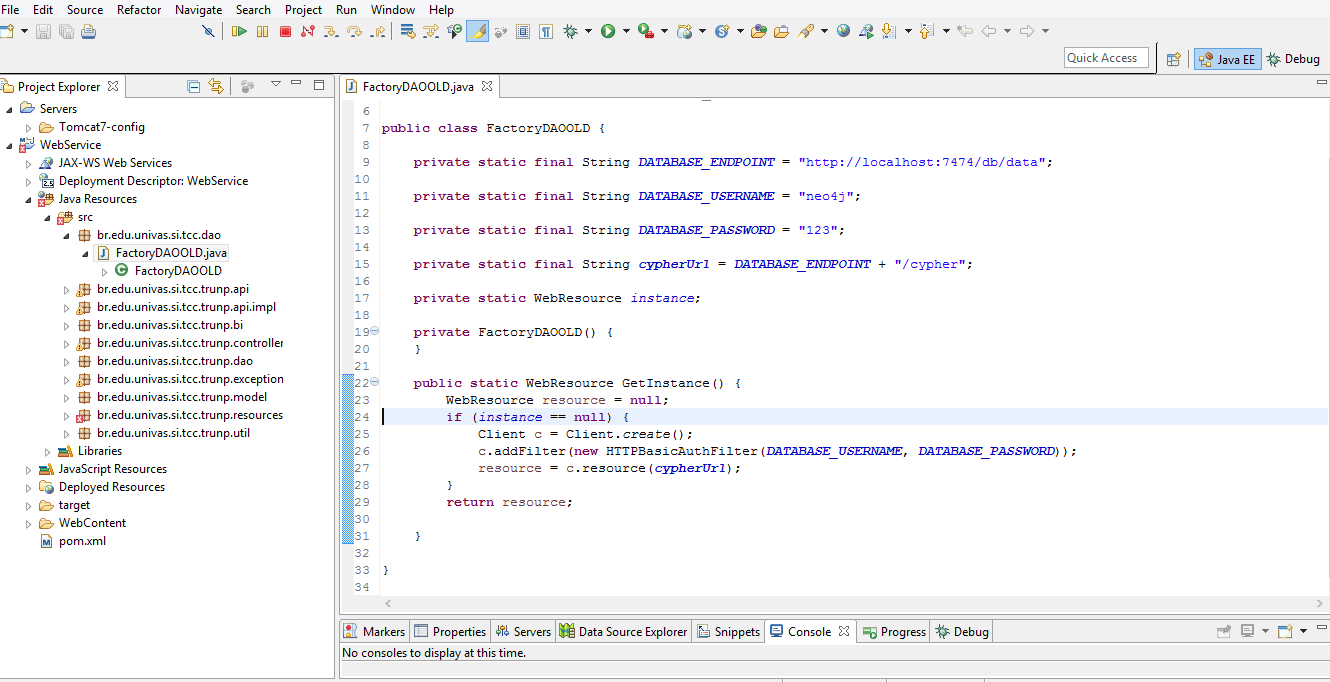
\includegraphics[scale=0.35]{./imagens/conexao-banco.jpg}}
	\caption[Código de comunicação com o banco]
	{Código de comunicação com o banco \textbf{Fonte:} Elaborado pelos autores.}
	\label{fig:exemplo1}
\end{figure}


\par A Figura 30 e 31 demonstram a tela inicial do banco de dados Neo4j e um exemplo de consulta realizada por meio da aplicação de gerencia da base de dados.

\begin{figure}[h!]
	\centerline{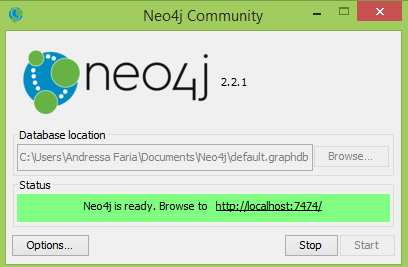
\includegraphics[scale=0.60]{./imagens/neo4j.jpg}}
	\caption[Tela de inicialização do Neo4j ]
	{Tela de inicialização do Neo4j \textbf{Fonte:} Elaborado pelos autores.}
	\label{fig:exemplo1}
\end{figure}

\begin{figure}[h!]
	\centerline{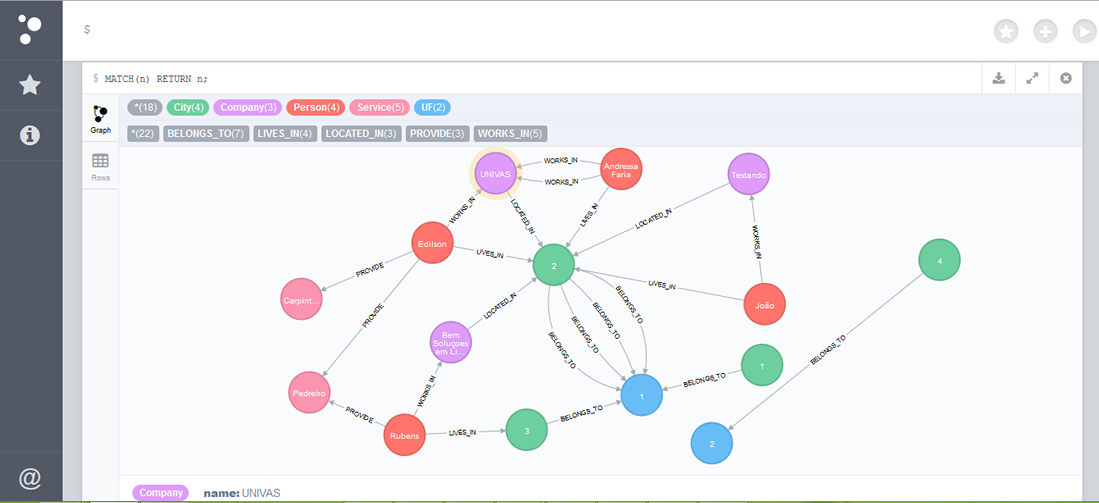
\includegraphics[scale=0.4]{./imagens/neo4j2.jpg}}
	\caption[Demonstração de uma consulta Cypher.]
	{Demonstração de uma consulta Cypher. \textbf{Fonte:} Elaborado pelos autores.}
	\label{fig:exemplo1}
\end{figure}
 
\newpage

\par Posterior a configuração do ambiente, iniciou-se o desenvolvimento propriamente dito. A princípio, utilizou-se as tecnologias Neo4j, sendo executado de forma \textit{embedded}, Primefaces e JSF. Porem não estava fluindo como o esperado, uma vez que o Neo4j utilizado desta maneira não permitia conectar ao sistema de gerenciamento da base de dados e abrir uma nova instancia de conexão simultânea, devido a limitações do próprio Neo4j, uma vez que um processo Java já ocupava tal conexão com o \textit{socket} do banco de dados.

\par Outro problema encontrado ao utilizar tais tecnologias foi que tanto a parte cliente (\textit{front end}) quanto a parte servidor (\textit{back end}) se encontravam totalmente acoplados em uma aplicação Java \textit{web}, portanto, a cada alteração realizada havia a necessidade de recompilar, construir e publicar a aplicação no servidor \textit{web}, impedindo que o desenvolvimento do \textit{software} fluísse, como era esperado. Por esses motivos decidiu-se mudar algumas das tecnologias utilizadas no \textit{front end} e, a maneira como o banco de dados era acessado até então. 

\par Posterior a esse incidente, passou a utilizar então as linguagens HTML 5, CSS 3, Java Script e Angular JS para auxiliar no desenvolvimento do \textit{front end}, ao invés de Primefaces e JSF. Para acesso ao banco de dados, lançou-se mão da forma \textit{embedded} e passou-se a utilizar a API REST disponibilizada pelo próprio banco. Tais decisões nos permitiram desacoplar o sistema e manter o \textit{front end} e o \textit{back end} independentes, evitando assim, que o mesmo problema voltasse a ocorrer. 

\par Após realizar a mudança de tecnologias, foi necessário realizar alguns testes para compreender o funcionamento do \textit{web service} REST e paralelamente foi feito o levantamento de materiais de referência do \textit{framework} Angular JS. Foi preciso realizar testes para validar a conexão com o banco de dados Neo4j via API REST, fornecida por ele. Também foram realizados testes para envio de requisições e recebimento de respostas do \textit{web service} REST, utilizando o Angular JS.

\par A partir deste ponto, a aplicação estava totalmente desacoplada, sendo necessário realizar uma configuração, a fim de permitir que as requisições enviadas pelo \textit{front end} fossem aceitas pelo \textit{back end}, localizado em outro domínio.

\par Devido a mudança de tecnologias já comentadas, houve-se a necessidade de atualizar os diagramas de sequencia e de classe, inserindo os contratos de serviços do \textit{web service} REST. Com a definição deste contrato, deu-se início ao desenvolvimento dos casos de uso, identificados na primeira fase do ICONIX. 

\par Posterior a realização dos testes e da escolha definitiva da arquitetura que seria utilizada, iniciou-se a implementação dos casos de uso. O primeiro a ser implementado foi o caso de uso de criação de conta. Para este caso de uso, teve-se o cuidado de criar um mecanismo de criptografia de dados sigilosos, como usuário e senha, visando garantir a segurança da aplicação. Estas informações criptografadas são enviadas a cada requisição e validadas pelo \textit{web service}, sendo atualizadas caso sejam válidas, tornado mais complexo a quebra desta criptografia. Este mecanismo foi desenvolvido com base no sistema de \textit{login} via \textit{token}. Segundo o embasamento usado na criação de contas, deu-se início ao desenvolvimento do sistema de \textit{login} e \textit{logoff}, que também utilizam o conceito de criptografia via \textit{token}. 

Imagem tela de login

\par Com o funcionamento do sistema de login, passou-se a desenvolver a página inicial da aplicação. Esta página contém as informações que são restritas ao usuário cadastrado, podendo ser eles: contratantes, provedores de serviço ou ambos. O sistema apresenta uma página inicial diferente para cada tipo de conta, contendo apenas as informações que são liberadas de acordo com o acesso do usuário, sendo essas informações relatórios, últimas atualizações na rede de parceiros, avaliações de serviços e prováveis parceiros.

imagem das 3 contas.

\par O caso de uso localizar parceiros foi desenvolvido após a conclusão do caso de uso criar conta. A lógica deste caso de uso consiste em localizar os possíveis parceiros, com base na rede de parceria do contrante.

imagem localizar parceiro



\par Ainda relacionado ao tipo de conta contratante ou ambos, foi implementado o caso de uso adicionar parceiro, que permite ao usuário convidar um possível parceiro para fazer parte da sua rede. Após a implementação da lógica para adicionar um novo parceiro, houve-se a necessidade de implementar o serviço de requisições de parcerias, uma vez que não bastava apenas um contratante convidar outro para se tornarem parceiros, mas sim que o contratante convidado aceitasse sua solicitação de parceria, para assim se tornarem parceiros. Visando disponibilizar estas solicitações de forma agradável ao usuário, foi desenvolvida uma funcionalidade para que o usuário pudesse aceitar ou rejeitar a solicitação enviada à ele.

imagem aqui :D

\par Após realizada a implementação do caso de uso adicionar parceiro, houve-se a necessidade de desenvolver a busca por todos os usuário que possuiam o tipo de conta contratante ou ambos e que possuiam um relacionamento de parceria com o usuário autenticado no sistema, além da funcionalidade de localizar novos parceiros, baseando-se na localização da empresa na qual o usuário trabalha e na cidade onde ele vive, sempre ordenando os resultados por meio da quantidade de parceiros em comum. 

\par O caso de uso gerenciar serviços foi implementado em sequência, abrangendo as principais funcionalidaes de gerenciamento: cadastrar e adicionar um novo serviço ao usuário, cujo tipo de conta é provedor de serviços, listar os serviços atribuídos a ele, e remover serviços quando necessário. Visando melhorar a usabilidade, foi implementado um mecanismo de busca, que permitiu filtrar os resultados por meio de um campo que possui a função  auto completar, evitando assim, possíveis erros e diminuindo o tempo gasto pelo usuário para adicionar o serviço. A função realiza a busca em uma lista de serviços anteriormente cadastrados, no entanto, caso não haja o serviço solicitado, o usuário tem a liberdade de cadastrá-lo e atribuí-lo a si mesmo.

\par A partir deste ponto, foi possível iniciar o desenvolvimento do caso de uso localizar mão de obra, uma vez que, este caso de uso dependia diretamente das implementações das funcionalidades adicionar parceiros para os usuários contratantes e adicionar serviços aos provedores de serviço. Para facilitar a localização e deixar o \textit{software} mais usual, esta busca se basea inicialmente no serviço buscado pelo usuário, sendo posteriormente modificada para também levar em consideração a funcionalidade avaliar serviço que foi implementada paralelamente. A avaliação de serviço permite ao contratante dar uma nota ao serviço que foi prestado a ele. Com estas informações foi possível desenvolver uma busca que levaria em consideração, além destas informações, a rede de parceiros do usuário contratante, a fim de lhe apresentar as melhores opções possíveis.

\par A fim de abranger a busca e possibilitar que novos prestadores de serviços sejam avaliados pelos contratantes, a consulta que antes apresentava apenas provedores de serviços que possuiam avaliações, sendo elas, positivas ou negativas, foi ampliada, possibilitando que profissionais não avaliados também entrassem na lista de prováveis provedores de serviços.

\par Para auxiliar na tomada de decisão do usuário contratante, foi implementada uma funcionalidade que realiza o cálculo da média de um determinado serviço prestado por um usuário provedor de serviço, tomando como base as avaliações da rede de parceiros do usuário autenticado, da empresa onde ele trabalha e da cidade onde vive, oferecendo assim uma forma simples de ter acesso a qualidade do serviço prestado. *******************************

\par Após realizada todas as implementações já descritas, houve-se a preocupação de desenvolver uma interface, que além de amigável fosse prática ao usuário, desta forma, foi disponibilizada algumas informações relevantes, que auxiliam o usuário a compreender o que está ocorrendo em sua rede de parceria. Como exemplo é possível citar a lista de parceiros em comum entre o usuário autenticado no sistema e um determinado contratante por meio da página de perfil dele.

\par A fim de agregar mais funcionalidades para o usuário provedor de serviços, foi criado na página inicial do \textit{software} uma funcionalidade que visa apresentar algumas dicas interessantes que contribui com a sua imagem perante ao \textit{software}, levando-o assim a obter uma quantidade maior de oportunidades de trabalho.

\par Para finalizar o desenvolvimento foram desenvolvidos gráficos que apresentam ao usuário informações a respeito da qualidade do serviço prestado pelo provedor de serviços, comparando-os com os demais prestadores.

\par Realizado todos os procedimentos apresentados nesta sessão foi possível obter como resultado final a conclusão deste trabalho.